\section{Pre-registration}\label{app:prereg}
The analysis plan (\texttt{docs/preregistration.md}) was committed to git before any canary-bearing model was
trained or scored. Commit \texttt{6ef2b5b} (Nov 10, 2026). The change log records two pre-result entries: the LR (App.~\ref{app:lr})
and 8 fictional entity names that also occur in the base corpus. Deviation after results: the ``stable'' minimum
dose used in the scorecard (Sec.~\ref{sec:results}), labelled exploratory. A third entry, written after the
160M results but before any 410M model was trained, fixes the 410M settings: same LR and analysis, batch
$2\times16$ for memory.

\section{Canary examples}\label{app:examples}
\todo{one example per type from data/canaries/mvr-v1.jsonl, rendered with zero-width characters shown as
$\langle$ZW$\rangle$.}

\section{Learning-rate selection}\label{app:lr}
Canary-free continued pretraining on 4.8M Wikipedia tokens; held-out loss on 50 unseen documents. bf16 autocast
inflated the loss and damaged the model, so the grid trains in tf32 and scores in fp32. Between the tf32 runs, the
larger LR was chosen, as pre-registered.

\begin{center}\small\IfFileExists{tables/app_lr.tex}{\begin{tabular}{lrrrr}
\toprule
Precision & LR & Held-out loss before & after & $\Delta$ \\
\midrule
tf32 & 1e-05 & 2.981 & 2.917 & -0.064 \\
tf32 & 3e-05 & 2.981 & 2.919 & -0.063 \\
bf16 & 1e-05 & 2.981 & 3.005 & +0.024 \\
bf16 & 3e-05 & 2.981 & 3.201 & +0.219 \\
bf16 & 1e-04 & 2.981 & 3.447 & +0.466 \\
\bottomrule
\end{tabular}
}{pending}\end{center}

\section{Numerical precision}\label{app:precision}
\todo{generated table: Pythia-160M loss in fp32 vs bf16 vs fp16 on 2048-token Wikipedia blocks, and on one short
sentence across CPU/A100/L40S.}

\section{Pipeline survival}\label{app:survival}
Planted copies still present (exact text; for fictional facts, entity and answer in the same document) after
each pipeline. The \emph{none} corpus has 82.5M tokens.

\begin{center}\small\setlength{\tabcolsep}{4pt}\IfFileExists{tables/app_survival.tex}{\begin{tabular}{lrrr}
\toprule
Type & substring dedup & NFKC & paraphrase 30\% \\
\midrule
Random seq. & 4.7\% (800/17,000) & 100.0\% (17,000/17,000) & 83.7\% (14,234/17,000) \\
Fluent trap & 4.5\% (766/17,000) & 100.0\% (17,000/17,000) & 69.5\% (11,823/17,000) \\
Watermark & 4.6\% (780/17,000) & 0.0\% (0/17,000) & 69.7\% (11,850/17,000) \\
Fictional fact & 99.9\% (16,983/17,000) & 100.0\% (17,000/17,000) & 99.9\% (16,987/17,000) \\
\midrule
Tokens & 77.5M & 82.1M & 82.3M \\
\bottomrule
\end{tabular}
}{pending}\end{center}

Per copy count. Under substring dedup, every canary keeps at most one copy, and all 1-copy random sequences
survive intact, so dedup and \emph{none} contain identical 1-copy canaries (Sec.~\ref{sec:results}).

\begin{center}\small\IfFileExists{tables/app_survival_dose.tex}{\begin{tabular}{lrrrr}
\toprule
Type & Copies & substring dedup & NFKC & paraphrase 30\% \\
\midrule
Random seq. & 1 & 200/200 & 200/200 & 166/200 \\
 & 4 & 200/800 & 800/800 & 658/800 \\
 & 16 & 200/3,200 & 3,200/3,200 & 2,661/3,200 \\
 & 64 & 200/12,800 & 12,800/12,800 & 10,749/12,800 \\
Fluent trap & 1 & 190/200 & 200/200 & 137/200 \\
 & 4 & 186/800 & 800/800 & 541/800 \\
 & 16 & 192/3,200 & 3,200/3,200 & 2,198/3,200 \\
 & 64 & 198/12,800 & 12,800/12,800 & 8,947/12,800 \\
Watermark & 1 & 190/200 & 0/200 & 138/200 \\
 & 4 & 192/800 & 0/800 & 563/800 \\
 & 16 & 199/3,200 & 0/3,200 & 2,232/3,200 \\
 & 64 & 199/12,800 & 0/12,800 & 8,917/12,800 \\
Fictional fact & 1 & 199/200 & 200/200 & 200/200 \\
 & 4 & 798/800 & 800/800 & 800/800 \\
 & 16 & 3,199/3,200 & 3,200/3,200 & 3,196/3,200 \\
 & 64 & 12,787/12,800 & 12,800/12,800 & 12,791/12,800 \\
\bottomrule
\end{tabular}
}{pending: run scripts/survival\_by\_dose.py}\end{center}

\section{All detectors}\label{app:all}
Primary detectors, every pipeline and dose (200 members vs.\ 200 non-members). Bold: $p<0.01$. Secondary
detectors are in \texttt{results/*/metrics.json}.

\paragraph{Pythia-160M.}
{\scriptsize\setlength{\tabcolsep}{4pt}\IfFileExists{tables/app_all_doses_p160m.tex}{\begin{tabular}{llrcccccc}
\toprule
 & & & \multicolumn{3}{c}{Gray box (loss)} & \multicolumn{3}{c}{Black box (completion)} \\
\cmidrule(lr){4-6}\cmidrule(lr){7-9}
Pipeline & Type & Copies & TPR & AUC & $p$ & TPR & AUC & $p$ \\
\midrule
none & Random seq. & 1 & 0.02 & 0.57 & \textbf{0.006} & 0.04 & 0.56 & \textbf{0.008} \\
 &  & 4 & 0.04 & 0.64 & \textbf{$2.9{\times}10^{-7}$} & 0.01 & 0.53 & 0.081 \\
 &  & 16 & 0.46 & 0.92 & \textbf{$3.2{\times}10^{-47}$} & 0.01 & 0.49 & 0.639 \\
 &  & 64 & 1.00 & 1.00 & \textbf{$2.4{\times}10^{-67}$} & 0.04 & 0.55 & 0.022 \\
 & Fluent trap & 1 & 0.04 & 0.55 & 0.048 & 0.00 & 0.51 & 0.330 \\
 &  & 4 & 0.01 & 0.65 & \textbf{$8.8{\times}10^{-8}$} & 0.01 & 0.47 & 0.831 \\
 &  & 16 & 0.53 & 0.95 & \textbf{$2.5{\times}10^{-55}$} & 0.05 & 0.51 & 0.347 \\
 &  & 64 & 1.00 & 1.00 & \textbf{$2.4{\times}10^{-67}$} & 0.18 & 0.73 & \textbf{$1.1{\times}10^{-15}$} \\
 & Watermark & 1 & 0.01 & 0.67 & \textbf{$4.0{\times}10^{-9}$} & 0.00 & 0.47 & 0.888 \\
 &  & 4 & 0.37 & 0.94 & \textbf{$1.5{\times}10^{-51}$} & 0.01 & 0.55 & 0.031 \\
 &  & 16 & 0.98 & 0.99 & \textbf{$3.1{\times}10^{-65}$} & 0.04 & 0.62 & \textbf{$1.7{\times}10^{-5}$} \\
 &  & 64 & 1.00 & 1.00 & \textbf{$2.4{\times}10^{-67}$} & 0.65 & 0.91 & \textbf{$1.9{\times}10^{-45}$} \\
 & Fictional fact & 1 & 0.01 & 0.57 & 0.011 & 0.00 & 0.51 & 0.191 \\
 &  & 4 & 0.01 & 0.52 & 0.298 & 0.00 & 0.52 & 0.063 \\
 &  & 16 & 0.10 & 0.66 & \textbf{$2.6{\times}10^{-8}$} & 0.00 & 0.51 & 0.064 \\
 &  & 64 & 0.20 & 0.88 & \textbf{$2.8{\times}10^{-40}$} & 0.00 & 0.51 & 0.251 \\
\midrule
substring dedup & Random seq. & 1 & 0.01 & 0.52 & 0.222 & 0.03 & 0.54 & 0.012 \\
 &  & 4 & 0.01 & 0.53 & 0.180 & 0.01 & 0.49 & 0.686 \\
 &  & 16 & 0.00 & 0.55 & 0.052 & 0.01 & 0.50 & 0.542 \\
 &  & 64 & 0.04 & 0.53 & 0.158 & 0.01 & 0.51 & 0.274 \\
 & Fluent trap & 1 & 0.01 & 0.56 & 0.026 & 0.01 & 0.50 & 0.439 \\
 &  & 4 & 0.00 & 0.52 & 0.261 & 0.01 & 0.48 & 0.743 \\
 &  & 16 & 0.02 & 0.50 & 0.453 & 0.01 & 0.54 & 0.093 \\
 &  & 64 & 0.02 & 0.54 & 0.066 & 0.04 & 0.50 & 0.546 \\
 & Watermark & 1 & 0.01 & 0.58 & \textbf{0.002} & 0.01 & 0.49 & 0.674 \\
 &  & 4 & 0.01 & 0.50 & 0.546 & 0.00 & 0.51 & 0.364 \\
 &  & 16 & 0.04 & 0.52 & 0.228 & 0.01 & 0.51 & 0.412 \\
 &  & 64 & 0.01 & 0.53 & 0.176 & 0.01 & 0.51 & 0.393 \\
 & Fictional fact & 1 & 0.00 & 0.57 & 0.011 & 0.01 & 0.50 & 0.332 \\
 &  & 4 & 0.01 & 0.52 & 0.273 & 0.00 & 0.51 & 0.121 \\
 &  & 16 & 0.06 & 0.67 & \textbf{$4.7{\times}10^{-9}$} & 0.00 & 0.51 & 0.157 \\
 &  & 64 & 0.17 & 0.88 & \textbf{$9.6{\times}10^{-41}$} & 0.00 & 0.52 & 0.033 \\
\midrule
NFKC & Random seq. & 1 & 0.01 & 0.57 & \textbf{0.008} & 0.01 & 0.58 & \textbf{$3.8{\times}10^{-4}$} \\
 &  & 4 & 0.11 & 0.65 & \textbf{$2.3{\times}10^{-7}$} & 0.01 & 0.48 & 0.743 \\
 &  & 16 & 0.45 & 0.91 & \textbf{$1.1{\times}10^{-45}$} & 0.03 & 0.51 & 0.365 \\
 &  & 64 & 1.00 & 1.00 & \textbf{$2.4{\times}10^{-67}$} & 0.12 & 0.59 & \textbf{$2.0{\times}10^{-4}$} \\
 & Fluent trap & 1 & 0.03 & 0.54 & 0.076 & 0.00 & 0.49 & 0.595 \\
 &  & 4 & 0.02 & 0.68 & \textbf{$6.8{\times}10^{-10}$} & 0.01 & 0.52 & 0.298 \\
 &  & 16 & 0.59 & 0.96 & \textbf{$1.7{\times}10^{-56}$} & 0.01 & 0.51 & 0.362 \\
 &  & 64 & 1.00 & 1.00 & \textbf{$2.4{\times}10^{-67}$} & 0.23 & 0.73 & \textbf{$5.9{\times}10^{-16}$} \\
 & Watermark & 1 & 0.01 & 0.50 & 0.449 & 0.01 & 0.53 & 0.178 \\
 &  & 4 & 0.01 & 0.60 & \textbf{$2.6{\times}10^{-4}$} & 0.01 & 0.47 & 0.880 \\
 &  & 16 & 0.12 & 0.70 & \textbf{$4.7{\times}10^{-12}$} & 0.01 & 0.51 & 0.416 \\
 &  & 64 & 0.33 & 0.80 & \textbf{$2.4{\times}10^{-25}$} & 0.12 & 0.63 & \textbf{$2.1{\times}10^{-6}$} \\
 & Fictional fact & 1 & 0.01 & 0.56 & 0.014 & 0.00 & 0.51 & 0.315 \\
 &  & 4 & 0.01 & 0.52 & 0.292 & 0.00 & 0.52 & 0.040 \\
 &  & 16 & 0.07 & 0.67 & \textbf{$5.2{\times}10^{-9}$} & 0.00 & 0.50 & 0.397 \\
 &  & 64 & 0.15 & 0.89 & \textbf{$1.5{\times}10^{-41}$} & 0.00 & 0.52 & 0.074 \\
\midrule
paraphrase 30% & Random seq. & 1 & 0.01 & 0.54 & 0.078 & 0.02 & 0.54 & 0.044 \\
 &  & 4 & 0.01 & 0.59 & \textbf{$6.6{\times}10^{-4}$} & 0.03 & 0.50 & 0.407 \\
 &  & 16 & 0.17 & 0.83 & \textbf{$3.5{\times}10^{-31}$} & 0.01 & 0.51 & 0.319 \\
 &  & 64 & 1.00 & 1.00 & \textbf{$2.4{\times}10^{-67}$} & 0.07 & 0.57 & \textbf{$9.6{\times}10^{-4}$} \\
 & Fluent trap & 1 & 0.01 & 0.50 & 0.514 & 0.01 & 0.52 & 0.244 \\
 &  & 4 & 0.03 & 0.58 & \textbf{0.002} & 0.02 & 0.48 & 0.786 \\
 &  & 16 & 0.20 & 0.81 & \textbf{$3.9{\times}10^{-27}$} & 0.04 & 0.52 & 0.278 \\
 &  & 64 & 0.99 & 1.00 & \textbf{$2.6{\times}10^{-67}$} & 0.06 & 0.60 & \textbf{$2.7{\times}10^{-4}$} \\
 & Watermark & 1 & 0.01 & 0.57 & \textbf{0.005} & 0.00 & 0.48 & 0.705 \\
 &  & 4 & 0.08 & 0.81 & \textbf{$8.2{\times}10^{-27}$} & 0.01 & 0.51 & 0.403 \\
 &  & 16 & 0.94 & 0.97 & \textbf{$2.3{\times}10^{-60}$} & 0.06 & 0.58 & \textbf{0.004} \\
 &  & 64 & 0.99 & 1.00 & \textbf{$3.0{\times}10^{-67}$} & 0.38 & 0.75 & \textbf{$5.4{\times}10^{-19}$} \\
 & Fictional fact & 1 & 0.01 & 0.56 & 0.017 & 0.01 & 0.50 & 0.496 \\
 &  & 4 & 0.00 & 0.51 & 0.366 & 0.00 & 0.51 & 0.241 \\
 &  & 16 & 0.07 & 0.67 & \textbf{$5.2{\times}10^{-9}$} & 0.01 & 0.50 & 0.496 \\
 &  & 64 & 0.15 & 0.88 & \textbf{$2.4{\times}10^{-40}$} & 0.00 & 0.50 & 0.506 \\
\bottomrule
\end{tabular}
}{pending}}

\paragraph{Pythia-410M.}
{\scriptsize\setlength{\tabcolsep}{4pt}\IfFileExists{tables/app_all_doses_p410m.tex}{\begin{tabular}{llrcccccc}
\toprule
 & & & \multicolumn{3}{c}{Gray box (loss)} & \multicolumn{3}{c}{Black box (completion)} \\
\cmidrule(lr){4-6}\cmidrule(lr){7-9}
Pipeline & Type & Copies & TPR & AUC & $p$ & TPR & AUC & $p$ \\
\midrule
none & Random seq. & 1 & 0.64 & 0.90 & \textbf{$1.4{\times}10^{-43}$} & 0.01 & 0.55 & 0.019 \\
 &  & 4 & 0.97 & 1.00 & \textbf{$1.3{\times}10^{-66}$} & 0.04 & 0.57 & \textbf{0.003} \\
 &  & 16 & 1.00 & 1.00 & \textbf{$2.4{\times}10^{-67}$} & 0.29 & 0.70 & \textbf{$9.1{\times}10^{-14}$} \\
 &  & 64 & 1.00 & 1.00 & \textbf{$2.4{\times}10^{-67}$} & 0.78 & 0.91 & \textbf{$6.2{\times}10^{-48}$} \\
 & Fluent trap & 1 & 0.09 & 0.74 & \textbf{$1.0{\times}10^{-16}$} & 0.01 & 0.53 & 0.124 \\
 &  & 4 & 0.71 & 0.97 & \textbf{$2.0{\times}10^{-59}$} & 0.07 & 0.57 & \textbf{0.009} \\
 &  & 16 & 1.00 & 1.00 & \textbf{$2.4{\times}10^{-67}$} & 0.35 & 0.76 & \textbf{$4.6{\times}10^{-19}$} \\
 &  & 64 & 1.00 & 1.00 & \textbf{$2.4{\times}10^{-67}$} & 0.93 & 0.98 & \textbf{$1.0{\times}10^{-63}$} \\
 & Watermark & 1 & 0.58 & 0.90 & \textbf{$2.0{\times}10^{-43}$} & 0.00 & 0.56 & 0.024 \\
 &  & 4 & 1.00 & 1.00 & \textbf{$2.4{\times}10^{-67}$} & 0.03 & 0.64 & \textbf{$1.1{\times}10^{-6}$} \\
 &  & 16 & 1.00 & 1.00 & \textbf{$2.4{\times}10^{-67}$} & 0.67 & 0.89 & \textbf{$3.2{\times}10^{-42}$} \\
 &  & 64 & 1.00 & 1.00 & \textbf{$2.4{\times}10^{-67}$} & 0.96 & 0.99 & \textbf{$1.3{\times}10^{-66}$} \\
 & Fictional fact & 1 & 0.00 & 0.61 & \textbf{$8.2{\times}10^{-5}$} & 0.01 & 0.50 & 0.419 \\
 &  & 4 & 0.01 & 0.62 & \textbf{$2.8{\times}10^{-5}$} & 0.01 & 0.51 & 0.323 \\
 &  & 16 & 0.17 & 0.83 & \textbf{$7.4{\times}10^{-30}$} & 0.01 & 0.53 & 0.017 \\
 &  & 64 & 0.64 & 0.98 & \textbf{$3.6{\times}10^{-61}$} & 0.02 & 0.53 & 0.016 \\
\midrule
substring dedup & Random seq. & 1 & 0.01 & 0.54 & 0.072 & 0.00 & 0.50 & 0.530 \\
 &  & 4 & 0.04 & 0.54 & 0.069 & 0.01 & 0.49 & 0.671 \\
 &  & 16 & 0.00 & 0.56 & 0.024 & 0.01 & 0.49 & 0.661 \\
 &  & 64 & 0.01 & 0.56 & 0.021 & 0.01 & 0.50 & 0.580 \\
 & Fluent trap & 1 & 0.02 & 0.54 & 0.088 & 0.01 & 0.49 & 0.613 \\
 &  & 4 & 0.00 & 0.54 & 0.076 & 0.01 & 0.48 & 0.784 \\
 &  & 16 & 0.04 & 0.55 & 0.042 & 0.00 & 0.50 & 0.558 \\
 &  & 64 & 0.02 & 0.56 & 0.014 & 0.01 & 0.50 & 0.486 \\
 & Watermark & 1 & 0.06 & 0.67 & \textbf{$9.0{\times}10^{-10}$} & 0.01 & 0.51 & 0.402 \\
 &  & 4 & 0.04 & 0.64 & \textbf{$3.0{\times}10^{-7}$} & 0.00 & 0.50 & 0.536 \\
 &  & 16 & 0.06 & 0.65 & \textbf{$1.2{\times}10^{-7}$} & 0.01 & 0.50 & 0.565 \\
 &  & 64 & 0.04 & 0.65 & \textbf{$1.1{\times}10^{-7}$} & 0.01 & 0.50 & 0.502 \\
 & Fictional fact & 1 & 0.01 & 0.61 & \textbf{$8.9{\times}10^{-5}$} & 0.01 & 0.50 & 0.409 \\
 &  & 4 & 0.04 & 0.62 & \textbf{$8.3{\times}10^{-6}$} & 0.00 & 0.50 & 0.501 \\
 &  & 16 & 0.18 & 0.84 & \textbf{$5.0{\times}10^{-32}$} & 0.01 & 0.53 & \textbf{0.009} \\
 &  & 64 & 0.62 & 0.98 & \textbf{$1.3{\times}10^{-62}$} & 0.02 & 0.55 & \textbf{$8.3{\times}10^{-4}$} \\
\midrule
NFKC & Random seq. & 1 & 0.58 & 0.88 & \textbf{$9.8{\times}10^{-41}$} & 0.01 & 0.54 & 0.047 \\
 &  & 4 & 0.90 & 0.98 & \textbf{$5.7{\times}10^{-63}$} & 0.01 & 0.56 & 0.011 \\
 &  & 16 & 1.00 & 1.00 & \textbf{$2.4{\times}10^{-67}$} & 0.14 & 0.69 & \textbf{$1.7{\times}10^{-12}$} \\
 &  & 64 & 1.00 & 1.00 & \textbf{$2.4{\times}10^{-67}$} & 0.79 & 0.92 & \textbf{$2.5{\times}10^{-49}$} \\
 & Fluent trap & 1 & 0.04 & 0.70 & \textbf{$7.3{\times}10^{-13}$} & 0.01 & 0.55 & 0.059 \\
 &  & 4 & 0.75 & 0.97 & \textbf{$4.8{\times}10^{-59}$} & 0.03 & 0.54 & 0.070 \\
 &  & 16 & 1.00 & 1.00 & \textbf{$2.4{\times}10^{-67}$} & 0.48 & 0.82 & \textbf{$1.1{\times}10^{-28}$} \\
 &  & 64 & 1.00 & 1.00 & \textbf{$2.4{\times}10^{-67}$} & 0.93 & 0.97 & \textbf{$1.3{\times}10^{-61}$} \\
 & Watermark & 1 & 0.04 & 0.56 & 0.027 & 0.01 & 0.52 & 0.200 \\
 &  & 4 & 0.12 & 0.77 & \textbf{$1.3{\times}10^{-20}$} & 0.00 & 0.51 & 0.386 \\
 &  & 16 & 0.62 & 0.93 & \textbf{$3.0{\times}10^{-51}$} & 0.07 & 0.54 & 0.078 \\
 &  & 64 & 0.85 & 0.99 & \textbf{$8.6{\times}10^{-64}$} & 0.23 & 0.71 & \textbf{$4.1{\times}10^{-13}$} \\
 & Fictional fact & 1 & 0.01 & 0.61 & \textbf{$7.3{\times}10^{-5}$} & 0.01 & 0.51 & 0.333 \\
 &  & 4 & 0.04 & 0.61 & \textbf{$5.4{\times}10^{-5}$} & 0.01 & 0.50 & 0.399 \\
 &  & 16 & 0.20 & 0.83 & \textbf{$1.1{\times}10^{-30}$} & 0.01 & 0.52 & 0.073 \\
 &  & 64 & 0.70 & 0.98 & \textbf{$1.9{\times}10^{-61}$} & 0.03 & 0.54 & \textbf{0.008} \\
\midrule
paraphrase 30% & Random seq. & 1 & 0.31 & 0.82 & \textbf{$1.3{\times}10^{-29}$} & 0.01 & 0.55 & 0.039 \\
 &  & 4 & 0.81 & 0.96 & \textbf{$1.4{\times}10^{-56}$} & 0.05 & 0.55 & 0.018 \\
 &  & 16 & 1.00 & 1.00 & \textbf{$2.4{\times}10^{-67}$} & 0.19 & 0.65 & \textbf{$3.2{\times}10^{-8}$} \\
 &  & 64 & 1.00 & 1.00 & \textbf{$2.4{\times}10^{-67}$} & 0.74 & 0.88 & \textbf{$1.5{\times}10^{-42}$} \\
 & Fluent trap & 1 & 0.04 & 0.61 & \textbf{$9.1{\times}10^{-5}$} & 0.01 & 0.51 & 0.350 \\
 &  & 4 & 0.19 & 0.84 & \textbf{$8.0{\times}10^{-33}$} & 0.01 & 0.52 & 0.290 \\
 &  & 16 & 0.99 & 1.00 & \textbf{$2.8{\times}10^{-67}$} & 0.14 & 0.63 & \textbf{$4.1{\times}10^{-6}$} \\
 &  & 64 & 1.00 & 1.00 & \textbf{$2.4{\times}10^{-67}$} & 0.80 & 0.93 & \textbf{$4.7{\times}10^{-51}$} \\
 & Watermark & 1 & 0.30 & 0.73 & \textbf{$2.3{\times}10^{-16}$} & 0.00 & 0.55 & 0.051 \\
 &  & 4 & 0.87 & 0.98 & \textbf{$9.4{\times}10^{-63}$} & 0.02 & 0.58 & \textbf{0.004} \\
 &  & 16 & 1.00 & 1.00 & \textbf{$2.4{\times}10^{-67}$} & 0.39 & 0.75 & \textbf{$9.0{\times}10^{-19}$} \\
 &  & 64 & 1.00 & 1.00 & \textbf{$2.4{\times}10^{-67}$} & 0.97 & 1.00 & \textbf{$7.1{\times}10^{-68}$} \\
 & Fictional fact & 1 & 0.01 & 0.60 & \textbf{$3.3{\times}10^{-4}$} & 0.01 & 0.51 & 0.147 \\
 &  & 4 & 0.03 & 0.61 & \textbf{$5.2{\times}10^{-5}$} & 0.01 & 0.51 & 0.258 \\
 &  & 16 & 0.12 & 0.81 & \textbf{$1.4{\times}10^{-27}$} & 0.01 & 0.52 & 0.057 \\
 &  & 64 & 0.68 & 0.97 & \textbf{$5.1{\times}10^{-59}$} & 0.01 & 0.54 & \textbf{0.006} \\
\bottomrule
\end{tabular}
}{pending}}

\section{False-positive check}\label{app:qq}
\begin{center}
  \IfFileExists{figs/fig4_qq.pdf}{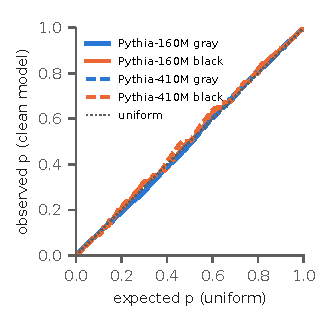
\includegraphics[width=0.4\linewidth]{figs/fig4_qq.pdf}}{\fbox{Fig 4 pending}}
  \captionof{figure}{Clean base models: p-values from 200 random re-splits per cell against the uniform
  distribution, for both primary detectors and both model sizes.}\label{fig:qq}
\end{center}
